
\begin{frame}{Symulacja robota}
%	zdjęcie Velmy w środowisku
	\begin{columns}
		\begin{column}{0.5\textwidth}
			\begin{itemize}
				\item Robot Velma - dwa manipulatory, każdy o siedmiu stopniach swobody
				
				
				\item Dostępne czujniki przydatne w nawigacji - dwa czujniki LiDAR, kamera Kinect, kamery rgb, czujnik inercji, czujniki odometrii na osiach bazy mobilnej (jedynie w prawdziwym robocie, symulacja oblicza odometrię w inny sposób)
				
			\end{itemize}
		\end{column}
		\begin{column}{0.5\textwidth}
%			\begin{center}
%				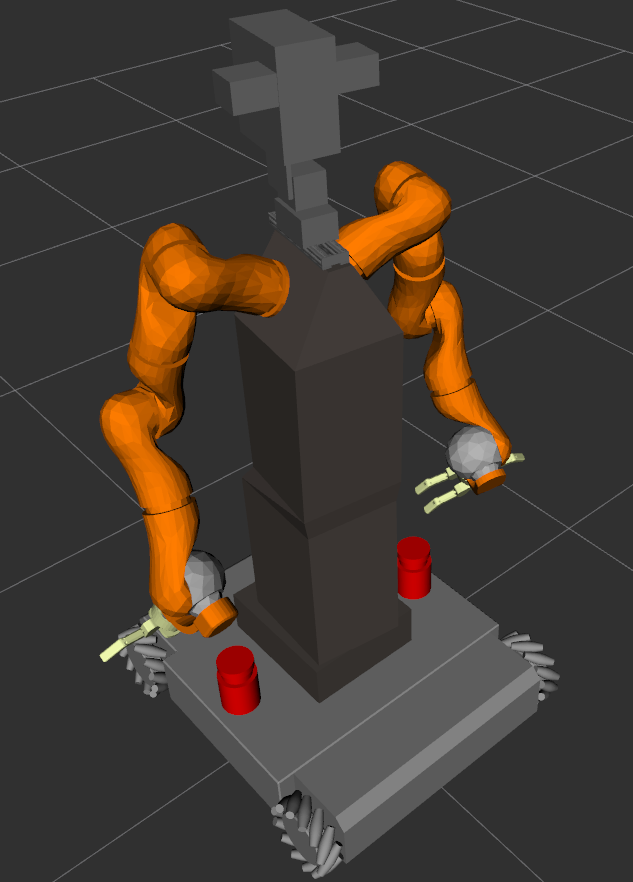
\includegraphics[height=0.5\textheight]{img/velma_wizualizacja.png} 
%			\end{center}
			\begin{itemize}
				\item Baza mobilna - wielokierunkowa, wykorzystująca koła szwedzkie
				\item Symulacja całego robota na potrzeby prac laboratoryjnych, w początkowych fazach projektów prace na samym robocie są zbyt niebezpieczne
			\end{itemize}
		\end{column}		
	\end{columns}
	
\end{frame}

\begin{frame}
\frametitle{Problemy z nawigacją robota Velma}
	\begin{itemize}
		\item należy wykrywać przeszkody znajdujące się wysoko ponad poziomem podłogi
		\item należy dobrać odpowiedni algorytm planowania i wykonania ścieżki wykorzystujący w pełni możliwości wielokierunkowej bazy mobilnej
		\item z powodu relatywnie skomplikowanej zasady działania napędu bazy mobilnej utrudnione jest zadanie precyzyjnego sterowania prędkością poruszania robota w środowisku
%TODO podać rozwiązanie problemów?
	\end{itemize}
\end{frame}

\begin{frame}
{Wykorzystywane narzędzia}
	\begin{columns}
		\begin{column}{0.25\textwidth}
			\begin{figure}
				\begin{center}
					
\includegraphics[width=\textwidth]{img/Ros_logo.png}
				\end{center}
			\end{figure}
		\end{column}
		\begin{column}{0.25\textwidth}  %%<--- here
						\begin{figure}
				\begin{center}
					
\includegraphics[width=\textwidth]{img/Gazebo_logo.png}		
				\end{center}
			\end{figure}
		\end{column}
				\begin{column}{0.25\textwidth}
			\begin{figure}
				\begin{center}
					
\includegraphics[width=\textwidth]{img/Python_logo.png}			
				\end{center}
			\end{figure}
		\end{column}
		\begin{column}{0.25\textwidth}  %%<--- here
						\begin{figure}
				\begin{center}
					
\includegraphics[width=\textwidth]{img/C++_Logo.png}
				\end{center}
			\end{figure}
		\end{column}
	\end{columns}
\footnotesize{Żródła: wikipedia.org, pngkey.com}
\end{frame}


\begin{frame}{Symulacja części mobilnej}
	\begin{columns}
		\begin{column}{0.5\textwidth}
			\begin{center}
				MODUŁ SYMULACYJNY
			\end{center}
			\begin{itemize}
				\item definicja kształtu wizualnego obiektów
				\item definicja kolizji obiektów
				\item definicja dynamiki obiektów
			\end{itemize}
			
		\end{column}
		\begin{column}{0.5\textwidth}  %%<--- here
			\begin{center}
				MODUŁ STERUJĄCY BAZY JEZDNEJ
			\end{center}
			\begin{itemize}
				\item wykorzystuje informacje o parametrach kolizji i dynamiki z pierwszego modułu
				\item przyjmuje jako wejście prędkość zadaną bazy
				\item oblicza siły działające na bazę
			\end{itemize}
		\end{column}
	\end{columns}
\end{frame}

\begin{frame}{Oprogramowanie części mobilnej}
	\begin{columns}
		\begin{column}{0.5\textwidth}
			\begin{center}
				ROS
			\end{center}
			\begin{itemize}
				\item popularny i rozwijany system programowania robotów
				\item umożliwia tworzenie niezależnych procesów w systemie operacyjnym komputera
				\item komunikacja między procesami z pomocą jednokierunkowych tematów i dwukierunkowych serwisów
			\end{itemize}
			
		\end{column}
		\begin{column}{0.5\textwidth}  %%<--- here
			\begin{center}
				GAZEBO
			\end{center}
			\begin{itemize}
				\item symulowanie obiektów w przestrzeni trójwymiarowej
				\item proste pisanie własnych wtyczek w C++
				\item początkowo część ROSa, teraz niezależna platforma
			\end{itemize}
		\end{column}
	\end{columns}
\end{frame}